% !TEX root = main.tex

\section{The Thin-Film Model}\label{sec:equations}
  In this model we consider a thin film of liquid on a flat surface with a free
  interface.
  This liquid is driven by gravity, shear and normal forces on the surface, and surface
  tension (see Figure~\ref{fig:thin_film}).
  We begin by considering the two dimensional incompressible Navier-Stokes equations,
  which have the form,
  \begin{align}
    u_x + w_z &= 0, \label{eq:incompressibility}\\
    \rho\p{u_t + u u_x + w u_z} &= -p_x + \mu \Delta u - \phi_x, \label{eq:con_mom1}\\
    \rho\p{w_t + u w_x + w w_z} &= -p_z + \mu \Delta w - \phi_z, \label{eq:con_mom2}
  \end{align}
  where \(\rho \) is the density, \(u\) is the horizontal velocity, \(w\) is the
  vertical velocity, \(p\) is the pressure, and \(\phi \) is the force of gravity.
  Equation~\eqref{eq:incompressibility} is the incompressibility condition and also
  represents conservation of mass.
  Equations~\eqref{eq:con_mom1} and~\eqref{eq:con_mom2} represent the conservation of
  momentum in the \(x\) and \(z\) directions respectively.
  We take a no penetration and no slip boundary condition at the lower boundary and the
  kinematic boundary condition at the upper boundary.
  These boundary conditions can be expressed as follows,
  \begin{align}
    w &= 0, \quad u = 0, &\text{at } z = 0, \\
    w &= h_t + u h_x, &\text{at } z = h,
  \end{align}
  where \(h\) is the height of the liquid.
  We can also describe the stress tensor, \(\v{T}\), at the free surface, \(z = h\),
  as
  \begin{align*}
    \v{T} \cdot \v{n} &= \p{-\kappa \sigma + \Pi_0}\v{n}
      + \p{\pd{\sigma}{s} + \tau_0}\v{t}, &\text{at } z = h,
  \end{align*}
  where \(\kappa \) is the mean curvature, \(\sigma \) is the surface tension, and
  \(\Pi_0 \) and \(\tau_0 \) are the normal and tangential components of the forcing
  respectively.

  \begin{figure}
    \centering
    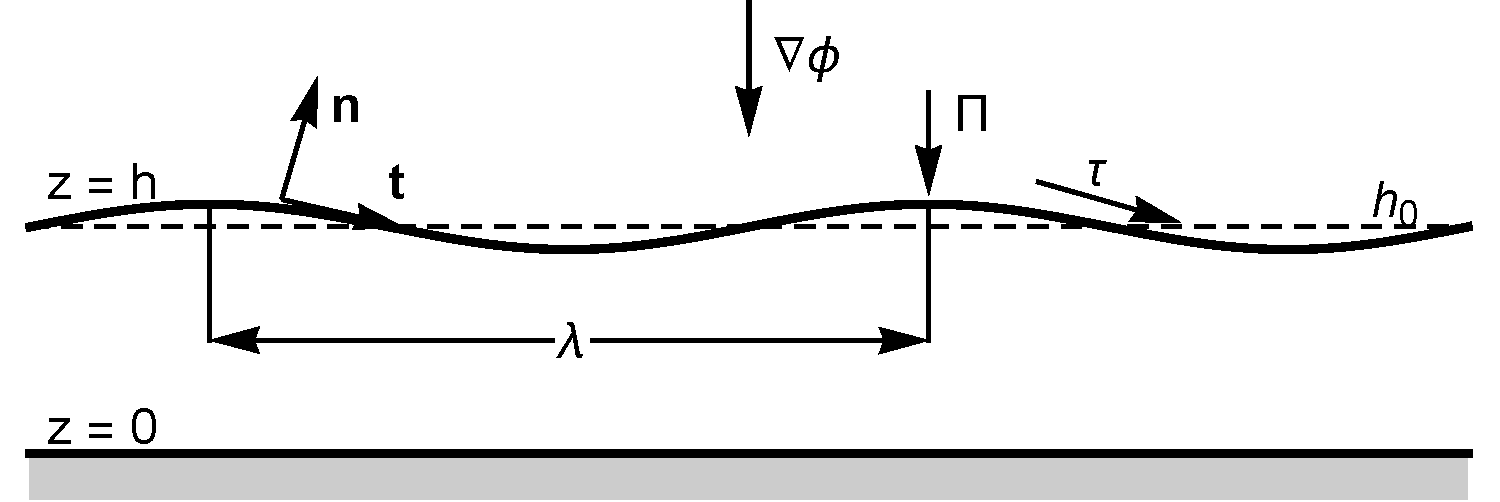
\includegraphics[scale=0.45]{figures/ThinFilm.pdf}
    \caption{A diagram of the Thin-Film Model}\label{fig:thin_film}
  \end{figure}

\subsection{Derivation}
  These equations completely describe the fluid, but we are now going to make a
  lubrication approximation, through a scaling argument similar to that given by Oron
  et al.~\cite{oron1997long}.
  For the lubrication approximation we are going to assume that the average height of
  the liquid, \(h_0\), is much smaller then the characteristic wavelength of the liquid,
  \(\lambda \).
  We will denote the ratio of these two lengths as \(\varepsilon \), that is
  \begin{equation}
    \varepsilon = \frac{h_0}{\lambda} \ll 1.
  \end{equation}
  Now we nondimensionalize the rest of the variables with respect to this ratio.
  We denote the nondimensional variables as the uppercase variables.
  As we stated earlier the characteristic height is \(h_0\) and the characteristic
  length is \(\lambda = h_0/\varepsilon \), so the nondimensional length variables are
  \begin{equation}
    Z = \frac{z}{h_0}, \quad X = \frac{\varepsilon x}{h_0}, \quad H = \frac{h}{h_0}.
  \end{equation}
  Let \(U_0\) be the characteristic horizontal velocity, then
  \begin{equation}
    \quad U = \frac{u}{U_0}, \quad W = \frac{w}{\varepsilon U_0},
  \end{equation}
  where the nondimensional vertical velocity, \(W\), follows from the continuity
  equation.
  It follows that time will be scaled by \(\lambda/U_0\), so nondimensional time is
  \begin{equation}
    T = \frac{\varepsilon U_0 t}{h_0}.
  \end{equation}
  Finally we assume that the flow is locally parallel or equivalently
  \(p_x \sim \mu u_{zz}\).
  This gives us the proper scaling for the pressure, gravity, and surface stresses,
  \begin{equation}
    P = \frac{\varepsilon h_0}{\mu U_0} p, \quad
    \Phi = \frac{\varepsilon h_0}{\mu U_0}\phi, \quad
    \Pi = \frac{\varepsilon h_0}{\mu U_0}\Pi_0, \quad
    \tau = \frac{h_0}{\mu U_0}\tau_0.
  \end{equation}
  Lastly we can nondimensionalize the surface tension as
  \begin{equation}
    \Sigma = \frac{\varepsilon \sigma}{\mu U_0}.
  \end{equation}
  Substituting these nondimensional variables into the original equations gives
  \begin{align}
    U_X + W_Z &= 0, \\
    \frac{\varepsilon U_0 \rho h_0}{\mu}\p{U_T + UU_X + WU_Z} &=
    -P_X + \p{\varepsilon^2 U_{XX} + U_{ZZ}} - \Phi_X, \\
    \varepsilon^3 \frac{\rho U_0 h_0}{\mu}\p{W_T + UW_X + WW_Z} &=
    -P_Z + \varepsilon^2\p{\varepsilon^2 W_{XX} + W_{ZZ}} - \Phi_Z,
  \end{align}
  at \(Z = 0\)
  \begin{gather}
    W = 0, \quad U = 0,
  \end{gather}
  and at \(Z = H\)
  \begin{gather}
    W = H_T + U H_x, \\
    -P - \Pi + \frac{2 \varepsilon^2}{1 + \varepsilon^2 H_X^2} \Big(\p{\varepsilon^2 H_X^2 U_X + W_Z} \nonumber \\
    - H_X \p{U_Z + \varepsilon^2 W_X}\Big) = \frac{\varepsilon^2 H_{XX}}{\p{1 + \varepsilon^2 H_X^2}^{3/2}} \Sigma, \\
    2 \varepsilon^2 H_X \p{W_Z - U_X} + \p{1 - \varepsilon^2 H_X^2} \p{U_Z + \varepsilon^2 W_X} \nonumber \\
    = \Sigma_X \p{1 + \varepsilon^2 H_X^2}^{1/2} + \tau \p{1 + \varepsilon^2 H_X^2}.
  \end{gather}

  We can now let \(\varepsilon \to 0\) which results in
  \begin{align}
    U_X + W_Z &= 0, \label{eq:nd_continuity}\\
    P_X + \Phi_X &= U_{ZZ}, \label{eq:nd_con_mom1} \\
    P_Z + \Phi_Z &= 0, \label{eq:nd_con_mom2}
  \end{align}
  at \(Z = 0\),
  \begin{gather}
    W = 0, \quad U = 0, \\
  \end{gather}
  and at \(Z = H\)
  \begin{align}
    W &= H_T + U H_x,  \\
    -P - \Pi &= \bar{\Sigma} H_{XX}, \\
    U_Z &= \Sigma_X + \tau.
  \end{align}
  Note that we assume that the surface tension is large, so that
  \(\bar{\Sigma} = \varepsilon^2 \Sigma = O(1)\).
  This is important in order to keep surface tension effects in the final equation.

  Lastly we integrate these equations over \(Z\) and apply the boundary conditions,
  in order to integrate out all of the variables except the free surface height, \(H\).
  Integrating equation~\eqref{eq:nd_continuity} gives
  \begin{equation}
    H_T + \pda{\dintt{0}{H}{U}{Z}}{X} = 0,
  \end{equation}
  and integrating equation~\eqref{eq:nd_con_mom1} twice gives
  \begin{equation}
    U = \p{\tau + \Sigma_X}Z + \p{P_X + \Phi_X}\p{\frac{1}{2} Z^2 - HZ},
  \end{equation}
  and finally integrating equation~\eqref{eq:nd_con_mom2} gives
  \begin{equation}
    P + \Phi = \eval{\Phi}{Z=H} - \Pi - \bar{\Sigma} H_{XX}.
  \end{equation}
  Substituting all of these equations together results in
  \begin{equation}
    H_T + \p{\frac{1}{2}\p{\tau + \Sigma_X}H^2 - \frac{1}{3}\p{\eval{\Phi}{Z=H} - \Pi}_X H^3}_X = - \p{\bar{\Sigma} H^3 H_{XXX}}_X.
  \end{equation}
  Setting all the constants to 1 and using the variable \(q\) instead gives us our
  original model equation~\eqref{eq:thin_film_model}.

\subsection{Hyperbolic Convection Dynamics}
  Consider the thin-film model with only the hyperbolic convection term, that is
  \begin{equation}
    q_t + \p{q^2 - q^3}_x = 0.
  \end{equation}
  Equations of the type \(q_t + f\p{q}_x = 0\) are known as conservation laws, where
  \(f\) is called the flux function.
  The dynamics of this equation are determined by the flux function.
  In the system case, the conservation law is called hyperbolic at \(q\) if \(f'(q)\)
  is diagonalizable with real eigenvalues.
  In the scalar case, this reduces to having a real valued flux function, so this term
  is indeed hyperbolic.
  We also need to consider if our flux function is convex or nonconvex.
  It is known that \(f\) is nonconvex if
  \(f''(q) = 0\) for some \(q\).
  In our case \(f''(q) = 2 - 6q\), so \(f''(q) = 0\) at \(q = \frac{1}{3}\).
  We can also see in Figure~\ref{fig:flux_function} that there is an inflection
  point at \(q = \frac{1}{3}\).
  Nonconvex flux functions can exhibit more complex behavior than convex flux
  functions.
  Nonconvex flux functions can involve compound waves including rarefaction-shocks.
  See Leveque~\cite{leveque2002finite} for more details.

  \begin{figure}
    \centering
    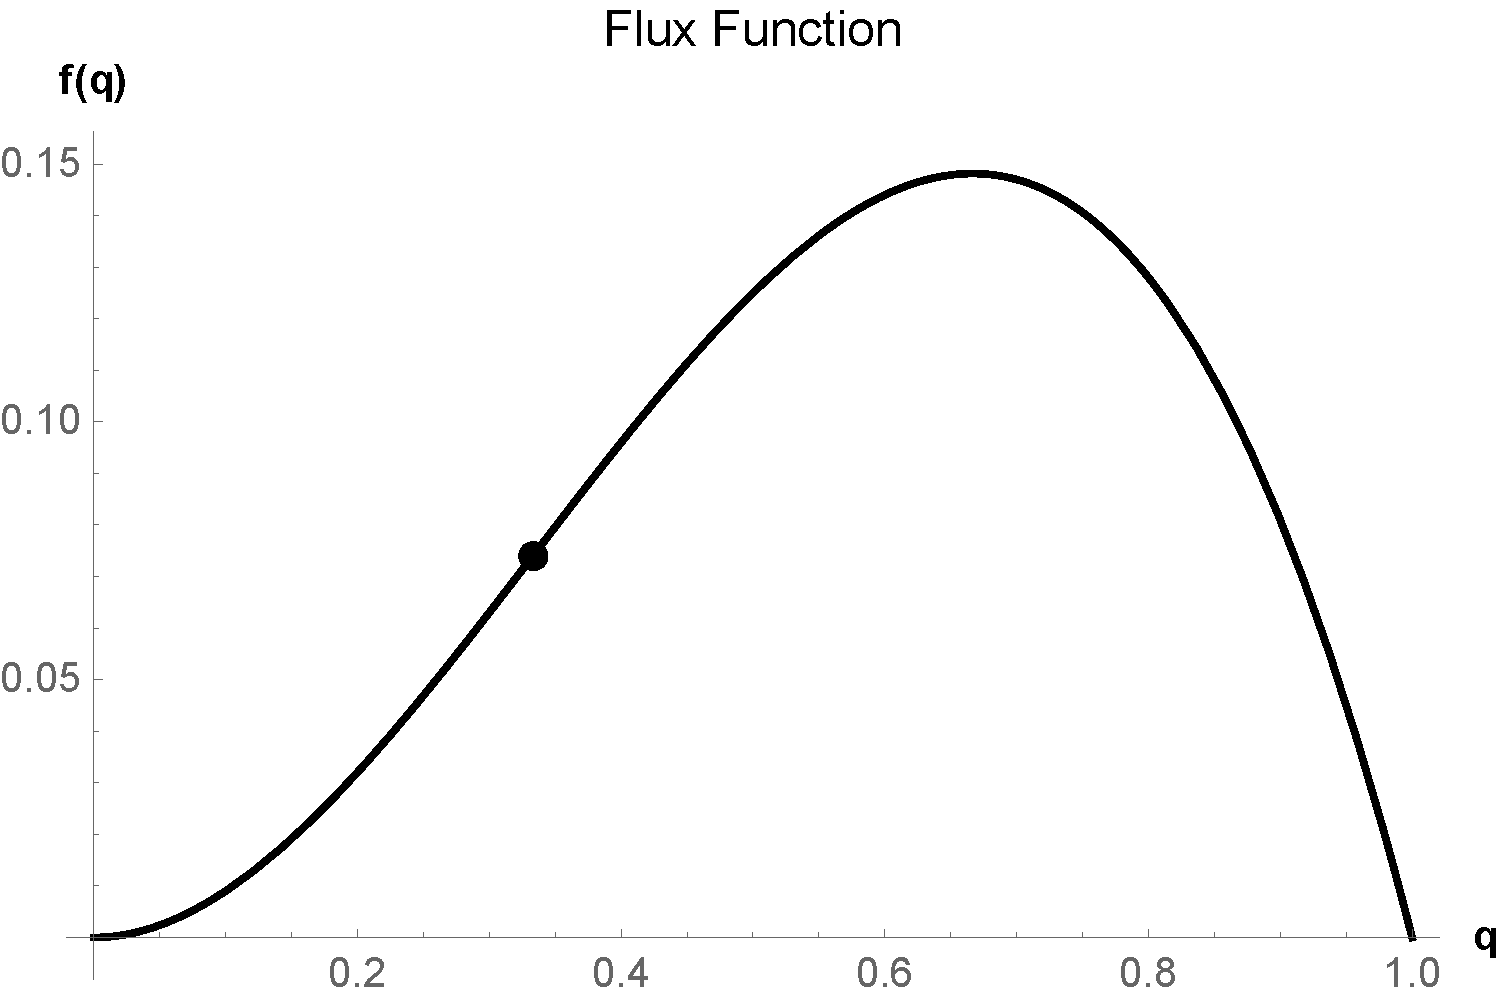
\includegraphics[scale=0.3]{figures/FluxFunctionNonconvex.pdf}
    \caption{Plot of flux function, \(f(q) = q^2 - q^3\).}\label{fig:flux_function}
  \end{figure}

  Another interesting feature of hyperbolic equations is that they have a finite
  wavespeed.
  The wavespeed of the conservation law is determined by \(f'(q)\).
  In our case, \(f'(q) = 2q - 3q^2\), so the wavespeed can be as large as
  \(\frac{1}{3}\).
  Having a finite wavespeed can be very useful for numerical methods, as this limits
  the speed of propagation of information.
  Each point in the domain has a finite radius of influence for each future time.

\subsection{Parabolic Dynamics}
  Now consider the thin-film model with only the parabolic term, that is
  \begin{equation}
    q_t = -\p{q^3 q_{xxx}}_x.
  \end{equation}
  Using the product rule of differentiation this is equivalent to
  \begin{equation}
    q_t = -\p{3q^2 q_x} q_{xxx} - q^3 q_{xxxx}.
  \end{equation}
  The dynamics of the third and fourth derivative terms can be analyzed with the
  Fourier transform.

  Consider, \(q_t = -q_{xxx}\), and take the Fourier transform of both sides, which
  results in
  \begin{equation}
    \mathcal{F}\p{q}_t = -i \xi^3 \mathcal{F}(q).
  \end{equation}
  Solving this ordinary differential equation (ODE) gives
  \begin{equation}
    \mathcal{F}\p{q} = e^{-i \xi^3 t}.
  \end{equation}
  We know that this type of solution has a dispersive dynamics.

  Similarly consider, \(q_t = -q_{xxxx}\), and take the Fourier transform of both sides.
  This gives the following ordinary differential equation
  \begin{equation}
    \mathcal{F}\p{q}_t = -\xi^4 \mathcal{F}(q).
  \end{equation}
  The solution to this ODE is
  \begin{equation}
    \mathcal{F}\p{q} = e^{-\xi^4 t}.
  \end{equation}
  This is a function that decays rapidly in time, and the higher the wavenumber,
  \(\xi \), the faster the diffusion.

  Therefore we expect this parabolic term to exhibit dispersive and diffusive dynamics.
  The dynamics are also nonlinearly coupled together making the behavior even more
  difficult to predict.
  The one thing that is clear is that the overall model is very stiff.
  The vast time scale difference between the finite wavespeed of the hyperbolic
  convection and the rapid decay of the nonlinear diffusion, make this model very stiff.
  Our numerical method must be able to handle this stiffness in a way that is not too
  computationally intensive.